\documentclass[a4paper,11pt]{article}
\pagenumbering{arabic}

\renewcommand*{\familydefault}{\sfdefault}
\renewcommand\footnotemark{}
\renewcommand\footnoterule{}

\setlength{\parindent}{0mm}
\setlength{\skip\footins}{0mm}
\setlength{\footnotesep}{0mm}

\usepackage[utf8]{inputenc} 
\usepackage[inner=20mm,outer=20mm,top=10mm,bottom=20mm,marginparsep=2mm,marginparwidth=8mm]{geometry}
\usepackage{t1enc}
\usepackage[magyar]{babel}
\usepackage{longtable}
\usepackage[usenames, dvipsnames]{xcolor}
\usepackage{colortbl}
\usepackage[colorlinks=true, linkcolor=blue]{hyperref}
\usepackage{enumitem}
\usepackage{pdfpages}
\usepackage{auto-pst-pdf}

\usepackage[nomessages]{fp}
\usepackage{multido}
\usepackage{pstricks}
\usepackage{caption}
\usepackage{xstring}
\usepackage{stringstrings}
\usepackage{ifthen}
\usepackage{xspace}
\usepackage{makeidx}
\usepackage{scalefnt}

\makeindex


\usepackage[nomessages]{fp}
\usepackage{multido}
\usepackage{pstricks}
\usepackage{caption}
\usepackage{xstring}
\usepackage{stringstrings}
\usepackage{ifthen}

\linethickness{0.01mm}

\newcommand\blfootnote[1]{%
  \begingroup
  \renewcommand\thefootnote{}\footnote{#1}%
  \addtocounter{footnote}{-1}%
  \endgroup
}

\newcommand{\HRule}{\rule{\linewidth}{0.5mm}}%

\newcommand{\FPmodulo}[2]{%
  \FPeval{\modulo}{trunc(#1-(#2*trunc(#1/#2,0)),0)}%
}%

\newcommand{\uind}[1]{%
  \raisebox{0.7ex}{{\scalefont{0.7}#1}}%
}%

\newcommand{\lind}[1]{%
  \raisebox{-0.4ex}{{\scalefont{0.7}#1}}%
}%

\newcommand{\notestr}[1]{%
  \IfDecimal{#1}{%
    \FPmodulo{#1}{12}%
    \FPeval{\noteposition}{trunc(\modulo,0)}%
    \substring[v]{CCDDEFFGGAAH}{\noteposition}{\noteposition}%
    \IfEq{\noteposition}{2}{\uind{$\sharp$}}{%
      \IfEq{\noteposition}{4}{\uind{$\sharp$}}{%
        \IfEq{\noteposition}{7}{\uind{$\sharp$}}{%
          \IfEq{\noteposition}{9}{\uind{$\sharp$}}{%
            \IfEq{\noteposition}{11}{\uind{$\sharp$}}{}}}}}%
  }{%
    \IfSubStr{#1}{bb}{%
      \StrSubstitute{#1}{bb}{}[\keya]%
      \keya\uind{$\flat\flat$}%
    }{%
      \IfSubStr{#1}{ss}{%
        \StrSubstitute{#1}{ss}{}[\keya]%
        \keya\uind{$\sharp\sharp$}%
      }{%
	\IfSubStr{#1}{b}{%
	  \StrSubstitute{#1}{b}{}[\keya]%
	  \keya\uind{$\flat$}%
	}{%
	  \IfSubStr{#1}{s}{%
	    \StrSubstitute{#1}{s}{}[\keya]%
	    \keya\uind{$\sharp$}%
	  }{#1}%
	}%
      }%
    }%
  }%
}%

\newcommand{\fretnote}[2]{%
  \IfDecimal{#1}{%
    \IfDecimal{#2}{%
      \FPeval{\noteposition}{trunc(#2 + #1*5 - trunc(#1/4,0) + 5,0)}%
      \snote{\noteposition}}{}}{}%
}%

\newcommand{\base}[2]{%
  \StrMid{#1}{2}{2}[\secondchar]%
  \StrMid{#1}{3}{3}[\thirdchar]%
  \IfSubStr{bs}{\thirdchar}{\StrLeft{#1}{3}[\keynote]}{\IfSubStr{bs}{\secondchar}{\StrLeft{#1}{2}[\keynote]}{\StrLeft{#1}{1}[\keynote]}}%
  \StrBehind{#1}{\keynote}[\chordid]%
  \IfSubStr{#2}{rmfamily}{\rmfamily\notestr{\ignorespaces\keynote\ignorespaces}}{}%
  \IfSubStr{#2}{textbf}{\textbf{\notestr{\ignorespaces\keynote\ignorespaces}}}{}%
  \normalfont%
  \StrSubstitute{\chordid}{b}{$\flat$}[\uida]%
  \StrSubstitute{\uida}{s}{$\sharp$}[\uidb]%
  \StrSubstitute{\uidb}{o}{\O}[\uidc]%
  \IfSubStr{\uidc}{mmaj}{%
    \StrSubstitute{\uidc}{mmaj}{maj}[\uidd]%
    \lind{m}\hspace*{-0.5ex}$\backslash$\hspace*{-0.5ex}\uind{\uidd}%
  }{%
    \IfSubStr{\uidc}{maj}{%
      \uind{\uidc}%
    }{%
      \IfSubStr{\uidc}{m}{%
        \StrSubstitute{\uidc}{m}{}[\uidd]%
        \IfStrEq{\uidd}{}{\lind{m}}%
        {\lind{m}\hspace*{-1.0ex}\uind{\uidd}}%
      }{%
        \uind{\uidc}%
      }%
    }%
  }%
}%

\newcommand{\note}[1]{%
  \notestr{#1}\normalfont%
}%

\newcommand{\snote}[1]{%
  \scalefont{0.6}\notestr{#1}%
}%

\newcommand{\key}[1]{%
  \base{#1}{rmfamily}%
}%

\newcommand{\chord}[1]{%
  \base{#1}{textbf}%
}%


\newcommand{\schord}[2]{%
  \chord{#1}/\hspace*{-0.5mm}\note{#2}%
}%

\newcommand{\scale}[2]{%
  \textit{\key{#1}} \textit{\rmfamily{#2}}\normalfont%
}%

\newcommand{\chordcircle}[3]{%
  \begin{pspicture}(3.5cm,3.5cm)%
  \def\cx{0}%
  \def\cy{5}%
  \def\outercircle{1.5}%
  \def\rnotecircle{0.23}%
  \FPeval{\innercircle}{\outercircle-\rnotecircle*2}%
  \pscircle[fillstyle=solid,linewidth=0.01,linecolor=black](\cx,\cy){\outercircle}%
  \pscircle[fillstyle=solid,linewidth=0.01,linecolor=black](\cx,\cy){\innercircle}%
  \multido{\i=270+30,\r=0+1 }{24}{%
    \FPeval{\z}{trunc(\r+1,0)}%
    \substring[q]{#1}{\z}{\z}%
    \FPeval{\octave}{\outercircle-trunc(\r/12, 0)*\rnotecircle*2}%
    \IfEq{\thestring}{.}{%
    \rput{-\i}(\cx,\cy){%
      \rput(\octave,0){%
        \pscircle[fillstyle=solid,linewidth=0.01,fillcolor=black]{0.05}%
      }%
    }%
    }{% 
      \rput{-\i}(\cx,\cy){%
        \rput(\octave,0){%
          \pscircle[fillstyle=solid,linewidth=0.01,linecolor=black]{\rnotecircle}%
        }%
      }%
      \rput{-\i}(\cx,\cy){%
        \rput{\i}(\octave,0){%
          {\snote{\z}}%
        }%
      }%
    }%
  }%
  \rput(\cx,\cy){\chord{#2#3}}%
  \end{pspicture}%
  \hspace*{8mm}%
  \vspace*{0.3mm}%
}%

\newcommand{\chordtable}[3]{%
  \begin{pspicture}(5cm,5cm)%
  \def\w{2.7}%
  \def\h{3.3}%
  \FPeval{\dw}{\w/5}%
  \FPeval{\dh}{\h/5}%
  \FPeval{\nx}{\w/2}%
  \FPeval{\ny}{\h+\dh/2}%
  \rput(\nx,\ny){\chord{#1}}%
  \FPeval{\nx}{\dw/-0.3}%
  \FPeval{\ny}{\dh*5}%
  \rput(\nx,\ny){\small $#2$}%
  \multido{\i=0+1}{6}{%
    \FPeval{\cx}{\i*\dw}%
    \FPeval{\cy}{\i*\dh}%
    \psline[linewidth=0.01](\cx,0)(\cx,\h)%
    \psline[linewidth=0.01](0,\cy)(\w,\cy)%
  }%
  \multido{\i=0+1}{30}{%
    \FPmodulo{\i}{6}%
    \FPeval{\st}{trunc(\modulo,0)}%
    \FPeval{\fr}{trunc(\i/6,0)}%
    \FPeval{\xpos}{\st*\dw}%
    \FPeval{\ypos}{4.5*\dh-\fr*\dh}%
    \FPeval{\fr}{trunc(#2 + \fr,0)}%
    \FPeval{\spos}{trunc(\i+1,0)}
    \substring[q]{#3}{\spos}{\spos}%
    \IfEq{\thestring}{.}{}{%
      \FPeval{\yu}{\ypos-\dh/4}%
      \FPeval{\yl}{\ypos+\dh/4}%
      \FPeval{\xs}{\xpos-\dw/2}%
      \FPeval{\xe}{\xpos+\dw/2}%
      \psframe[fillstyle=solid,fillcolor=white,linecolor=white](\xs,\yu)(\xe,\yl)%
      \IfEq{\thestring}{-}{%
        \psline[linewidth=0.03](\xs,\yu)(\xe,\yu)%
        \psline[linewidth=0.03](\xs,\yl)(\xe,\yl)%
      }{%
        \IfEq{\thestring}{X}{%
          \rput(\xpos,\ypos){X}%
        }{%
          \rput(\xpos,\ypos){\small\textbf{\thestring}\fretnote{\st}{\fr}}%
          \psline[linewidth=0.03](\xs,\yu)(\xe,\yu)%
          \psline[linewidth=0.03](\xs,\yl)(\xe,\yl)%
        }%
      }%
    }%
  }%
  \end{pspicture}%
  \hspace*{8mm}%
  \vspace*{0.3mm}%
}%

\newcommand{\fretboard}[3]%
{%
  \ifthenelse{\equal{#1}{}}{}{%
    \ifthenelse{\equal{#2}{}}{%
      \vspace*{1mm}#1~\\\vspace*{1mm}%
    }{}}%
  \begin{pspicture}(\linewidth,2.5cm)%
  \def\frets{16}%
  \def\dx{1.0}%
  \def\dy{0.4}%
  \def\disp{0.3}%
  \FPeval{\midy}{\dy * 2}%
  \FPeval{\notes}{trunc(\frets * 6,0)}%
  \FPeval{\sys}{0 - \dy/2 - 0.05}%
  \FPeval{\sye}{5*\dy - \dy/2 + 0.05}%
  \FPeval{\sxs}{\dx - \disp}%
  \multido{\i=0+1}{\frets}{%
    \FPeval{\sxs}{\i*\dx + \dx - \disp}%
    \psline[linewidth=0.01](\sxs,\sys)(\sxs,\sye)% 
    \ifthenelse{\equal{\i}{5}}{%
      \FPeval{\dotx}{\sxs - \dx*0.5}%
      \pscircle[fillstyle=solid, fillcolor=gray, linecolor=gray](\dotx,\midy){0.1}%
    }{}%
    \ifthenelse{\equal{\i}{7}}{%
      \FPeval{\dotx}{\sxs - \dx*0.5}%
      \pscircle[fillstyle=solid, fillcolor=gray, linecolor=gray](\dotx,\midy){0.1}%
    }{}%
    \ifthenelse{\equal{\i}{0}}{%
      \psline[linewidth=0.06](\sxs,\sys)(\sxs,\sye)% 
    }{}%
    \ifthenelse{\equal{\i}{12}}%
    {%
      \psline[linewidth=0.06](\sxs,\sys)(\sxs,\sye)% 
    }{}%
  }%
  \multido{\i=0+1}{6}%
  {%
    \FPeval{\sys}{\i*\dy - \dy/2}%
    \FPeval{\str}{0.04 - \i*0.005}%
    \psline[linewidth=0.01](0,\sys)(\textwidth,\sys)%
  }%
  \multido{\i=0+1}{\notes}%
  {%
    \FPmodulo{(\i)}{\frets}%
    \FPeval{\disp}{trunc(\frets*(5-trunc(\i/\frets,0)) + \modulo + 1,0)}%
    \substring[q]{#3}{\disp}{\disp}%
    \FPmodulo{(\i)}{\frets}%
    \IfEq{\thestring}{.}{}%
    {%
      \FPeval{\fre}{\modulo}%
      \FPeval{\stri}{trunc(\i/\frets,0)}%
      \FPeval{\xc}{\dx*\fre + 0.05}%
      \FPeval{\yc}{\dy*(\stri - \dy/2)}%
      \rput[tl](\xc,\yc){%
        \psframebox[fillstyle=solid,linecolor=white,framesep=0]{%
          \IfEq{\thestring}{x}{%
            \fretnote{\stri}{\fre}%
          }{%
            \small\textbf{\thestring}\fretnote{\stri}{\fre}%
          }%
        }%
      }%
    }%
  }%
  \end{pspicture}~\\%
  \ifthenelse{\equal{#1}{}}{}{%
    \ifthenelse{\equal{#2}{}}{}{%
      \vspace{-0.8cm}%
      \captionof{figure}{#1}%
      \label{#2}%
      \vspace{0.3cm}%
    }%
  }%
}%

\newcommand{\ideasubsection}[1]{%
  \subsection*{\raisebox{-0.5ex}{\includegraphics[width=5mm]{./images/idea.pdf}}~~#1}
}

%chord shortcuts
\def\Amaj{\chord{A}}
\def\Amin{\chord{Am}}

 
% packed itemization with caption and label
\newenvironment{pitemize}[2][]%
{%
  \def\arg{}%
  \def\tit{}%
  \ifx&#1&%
  \else%
    \ifx&#2&%
     \def\tit{~\\#1}%
    \else%
     \def\arg{\captionof{table}{#1}\label{#2}}%
    \fi%
  \fi%
  \addtocounter{table}{-1}%
  \tit%
  \begin{longtable}[l]{lllllllllllllllllll}%
}{%
  \end{longtable}%
  \arg%
}%

% packed enumeration
\newenvironment{penumerate}%
{%
  \begin{enumerate}[leftmargin=0.5cm]%
  \setlength{\itemsep}{1pt}%
  \setlength{\parskip}{0pt}%
  \setlength{\parsep}{0pt}%
}{%
  \end{enumerate} %
}%

% chord type table
\newenvironment{chords}[1]%
{
  \begin{longtable}[l]{|p{40mm}|p{15mm}||p{5mm}|p{5mm}|p{5mm}|p{5mm}|p{5mm}|p{5mm}|p{5mm}|p{5mm}|p{5mm}|p{5mm}|p{5mm}|p{5mm}|} %
  \hline %
  \textbf{#1} & \textbf{Jel} & p & k2 & n2 & k3 & n3 & t4 & sz5 & t5 & k6 & n6 & k7 & n7 \\ %
  \hline %
  \endhead %
}%
{%
  \hline %
  & \textbf{Jel} & p & k2 & n2 & k3 & n3 & t4 & sz5 & t5 & k6 & n6 & k7 & n7 \\ %
  \hline %
  \end{longtable} %
}%

% section excercises
\newenvironment{practices}%
{%
  \subsection*{\raisebox{-0.5ex}{\includegraphics[width=12mm]{./images/practice.pdf}}~~Gyakorlatok}%
  \begin{penumerate} %
}%
{%
  \end{penumerate} %
}%

% Music notation
\newcommand{\aisz}{$A^\sharp$\xspace}
\newcommand{\gisz}{$G^\sharp$\xspace}
\newcommand{\cisz}{$C^\sharp$\xspace}
\newcommand{\disz}{$D^\sharp$\xspace}
\newcommand{\fisz}{$F^\sharp$\xspace}
\newcommand{\asz}{$A^b$\xspace}
\newcommand{\bebe}{$B^b$\xspace}
\newcommand{\desz}{$D^b$\xspace}
\newcommand{\esz}{$E^b$\xspace}
\newcommand{\gesz}{$G^b$\xspace}
\def\sdim{\oslash\xspace}
\def\dim{O\xspace}
\newcommand{\sst}{$\frac{1}{2}$}
 
\graphicspath{ {../rajz/} }

\begin{document}
%\input{./titlepage.tex}

\tableofcontents

\clearpage

\section{Bevezetés}
\label{sec:bevezetes}
Az átalakítás célja a társasházi lakás energiafelhasználásának és szén-dioxod kibocsátásának csökkentése.
A beépítendő elemek kiválasztásánál lényeges szempont a hosszú, karbantartásmentes rendelkezésreállás és az energiatakarékos üzem.
A következő fejezetekben az átalakítás egymással összefüggő lépései, a kivitelezés időterve és költségvetése olvasható.
A dokumentumnak szintén célja kivitelezők tájékoztatása és munkájuk összehangolása. 

\section{Földgáz üzemű készülékek cseréje}
\label{sec:foldgazcsere}
A lakás jelenlegi fűtését két darab parapet kéményes gázkonvektor biztosítja.
A melegvízellátásról nyílt égésterű átolyó vízmelegítő gondoskodik. 
A főzés és sütés is földgázzal történik. 
A világítás jelenleg is energiatakarékos, kompakt fénycsöves. \\

A földgáz üzemű készülékek üzemeltetése jelenleg olcsóbb az elektromos megfelelőjüknél.
Ugyanakkor hatásfokuk kisebb. A robbanásveszélyes földgáz égéstermékének eltávolításával a
megtermelt hő egy része is távozik a lakótérből. Emellet a füstgáz üvegházhatású összetevőket tartalmaz.
A nyílt égésterű készülékek miatt a falon légbeeresztő van kialakítva, ami a statikus kéményhuzat miatt
folyamatos légcserét okoz. \\

A terv szerint a gázvételezés a lakásban megszűnik és az így kieső szolgáltatásokat takarékos
elektromos készülékek biztosítják majd. Ezek az előző sorrenben: infra fűtőfilmes mennyezetfűtés, 
villamos bojler, indukciós főzőlap és elektromos sütő. \\

A pályázat része az előbb említett berendezések működési feltételeinek biztosítása és 
tartószerkezetének kivitelezése is. Ez a fűtőfólia esetében direkt függesztett, síkvázas 
impregnált gipszkarton álmennyezet kialakítását jelenti.
Az álmennyezet illetve a fűtőfólia hatékony elhelyezéséhez szükséges néhány vékony 
közfal eltávolítása is (\ref{fig:bontas}. ábra). A költségvetésnek nem része, de szükséges
a \ref{fig:alaprajz}. ábrán látható gipszkarton válaszfalak felépítése is.
A többi berendezés esetében a működési feltételek a villamos- és víz bekötések megfelelő kialakításával biztosíthatók. \\

Az energiafelhasználás további csökkentése érdekében kompakt fénycsöves világítást az álmennyezetbe 
épített LED világítótestek váltják fel.

\subsection{Villamos teljesítmény bővítés}
A lakás jelenlegi villamos hálózatát 1x20A kismegszakító védi.
Az új fogyasztók bekötéséhez ezt szükséges 3x32A-re bővíteni.
Az épület 1969-es felállításakor elvárható lakás villamos hálózat sajnos szintén nem felel meg az átlakított 
rendszernek, ezért a későbbiekben részletezett gipszkarton álmennyezet alatt új, célirányos
vezetékezést kell kialakítani. Szintén szükséges új lakáselosztó kialakítása
megfelelő megfelelő számú és értékű áramkör- és életvédelmi berendezésekkel.

\subsection{Megújuló energia felhasználása}
\label{sec:napelem}
A villamos energia felhasználásának kedvező vonatkozása, hogy a megújuló forrásból megtermelt 
energia, -- esetünkben napenergia -- könnyen bevonható a környezet megóvása és a költségek csökkentése 
érdekében.

\section{Energiafelhasználás csökkentése}
\label{sec:hoatbocsatas}
A terv része a lakás hőveszteségének illetve gépi hűtés szükségleténak csökkentése is.

\subsection{Szigetelés}
\label{sec:burkolat}
A földgáznál költségesebb villamos energia hatékony felhasználása érdekében szükséges a jelenlegi födém és
a környezettel határos falazat szigetelésének javítása. A nedves helyiségek belső- illetve az erkély nappalival 
határos külső falain 40mm XPS lap, a száraz helyiségekben 12mm IsoTex lap kerül felragasztásra (\ref{fig:szigeteles}. ábra). \\

A födém hőszigetelésén az előzőekben említett infra fűtőfilm rétegrendjéhez tartozó, gipszkarton takarás alá
fektetett 50mm kőzetgyapot paplan és hőtükör fólia javítja.

\subsection{Hővisszanyerő gépi szellőztetés}
\label{sec:szellozo}
A párazáró szigetelés és a már beszerelt passzív ház minőségű műanyag nyílászárók miatt egészségtelen szintre nő
a lakótér páratartalma és $CO_2$ szintje, valamint a hideg felületeken télen penész képződés indul meg. A gyakori szellőztetés ezt
nem oldja meg, ugyanakkor számos kedvezőtlen hatása van. Az energiahatékonyság romlik, a nyílászárók minősége
a gyakori működtetéstől szintén csökken. A külső levegővel por kerül a belső térbe, ami gyakoribb takarításhoz,
több energia és vegyszer felhasználásához vezet. \\

A gépi szellőzető a nedves helyiségekből elszívott levegő hőjét átadja a kívülről, szűrőn keresztül 
beszívott friss levegőnek. A felmelegített friss levegő a száraz helyiségekbe kerül, míg az elhasznált levegő
a szabadba távozik. A friss levegő ellátás és a használt levegő eltávolítás a homlokzaton kialakítandó D125
fal áttöréseken keresztül történik majd. \\

A berendezés működéséhez szükséges légtechnikai csövezés a gipszkarton álmennyezet alatt kerül elhelyezésre.

\subsection{Árnyékolás}
\label{sec:arnyekolas}
Automatizálható motoros árnyékolókkal tovább javítható a nyílászárók hőszigetelése, vagy nyáron 
szükségelenné tehető a klímaberendezés üzemeltetése.

\section{Kivitelezés}
\label{sec:sorrend}
A kivitelezés lépései egymásra épülnek, ezért sorrendjük az alábbi ütemterv szerint alakítandó.

\section{Költségvetés}
\label{sec:koltsegvetes}
A kivitelezés lépései egymásra épülnek, ezért sorrendjük az alábbiak szerint alakítandó.

\clearpage
\section{Táblázatok}
\label{sec:tablazatok}

\clearpage
\section{Ábrák}
\label{sec:abrak}
\begin{figure}[h]
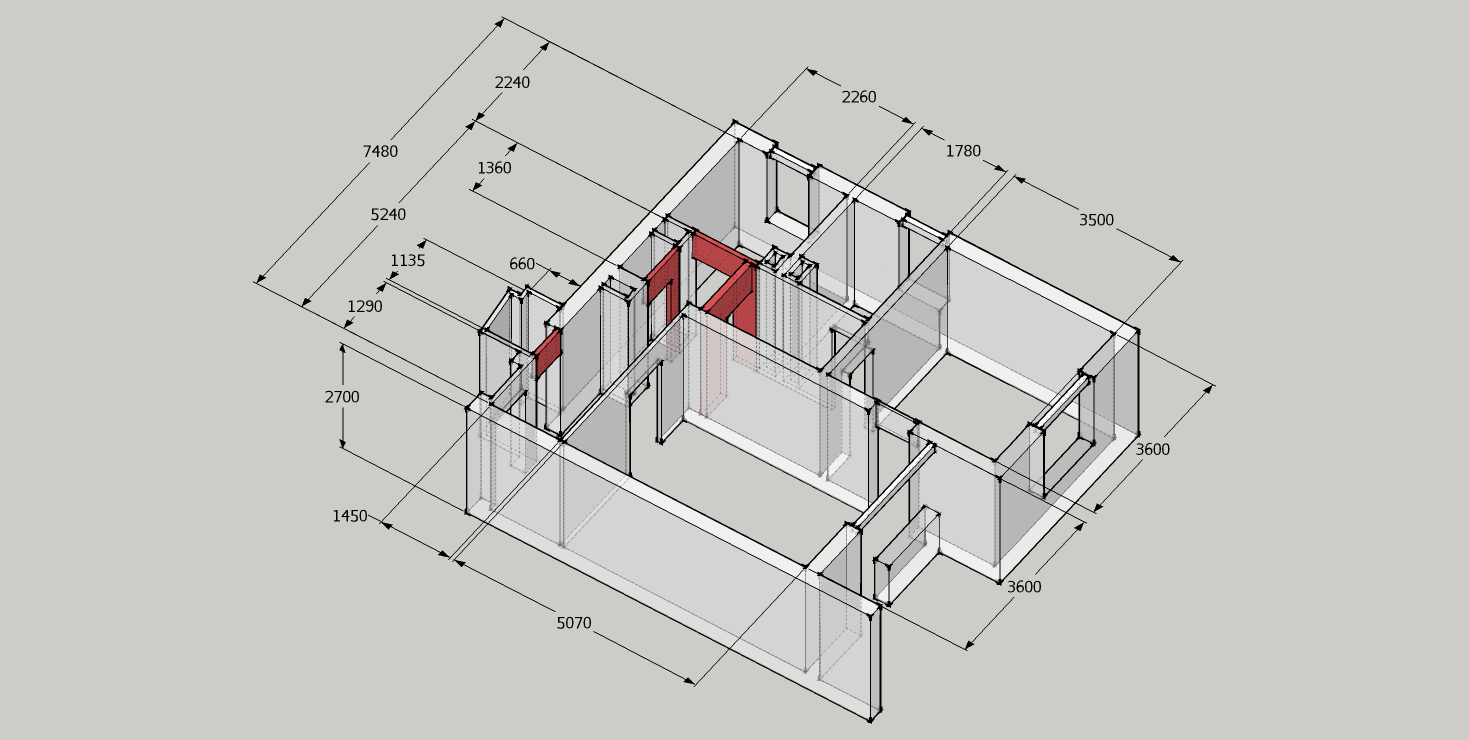
\includegraphics[width=\textwidth]{bontas.png}
\caption{Falazat bontott részei}
\label{fig:bontas}
\end{figure}
\begin{figure}[h]
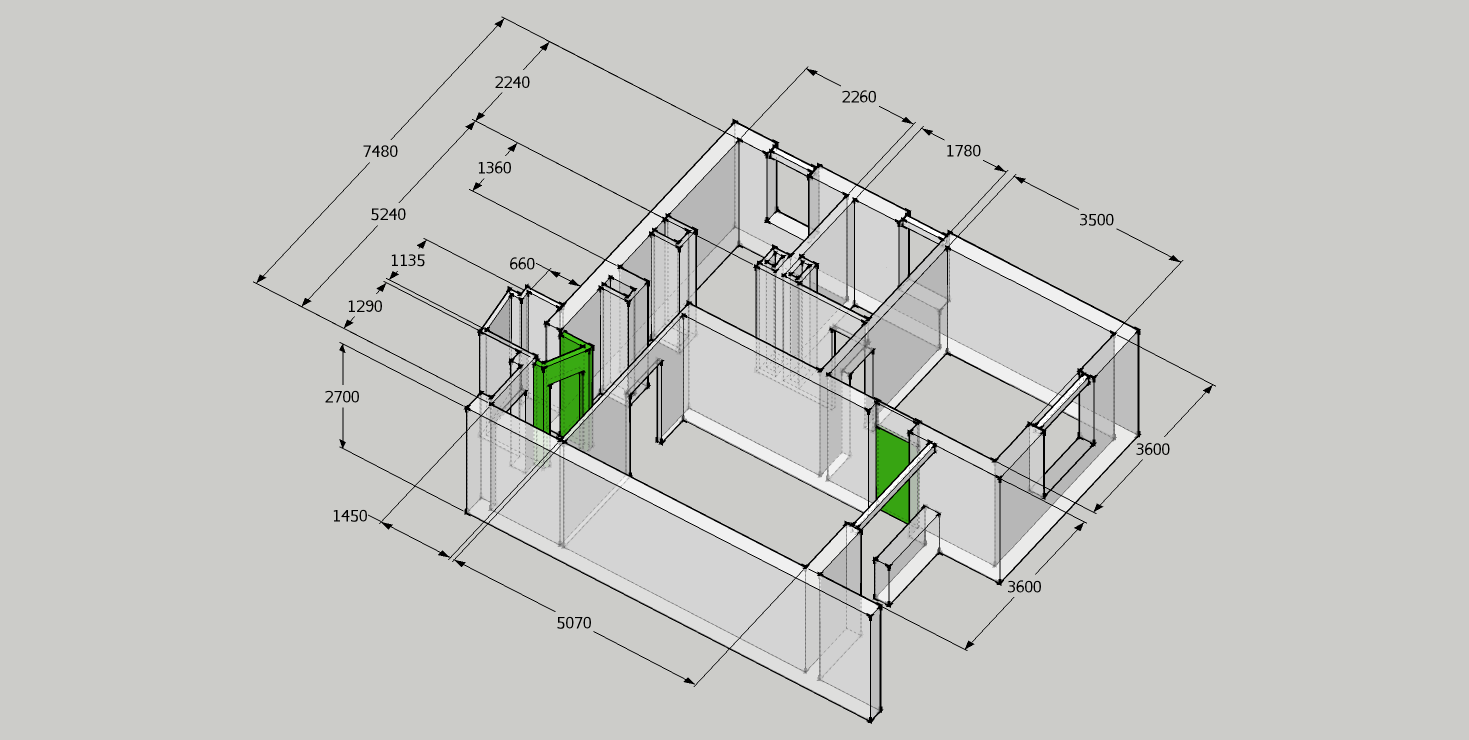
\includegraphics[width=\textwidth]{alaprajz.png}
\caption{Felújításra kész falazat}
\label{fig:alaprajz}
\end{figure}
\begin{figure}[h]
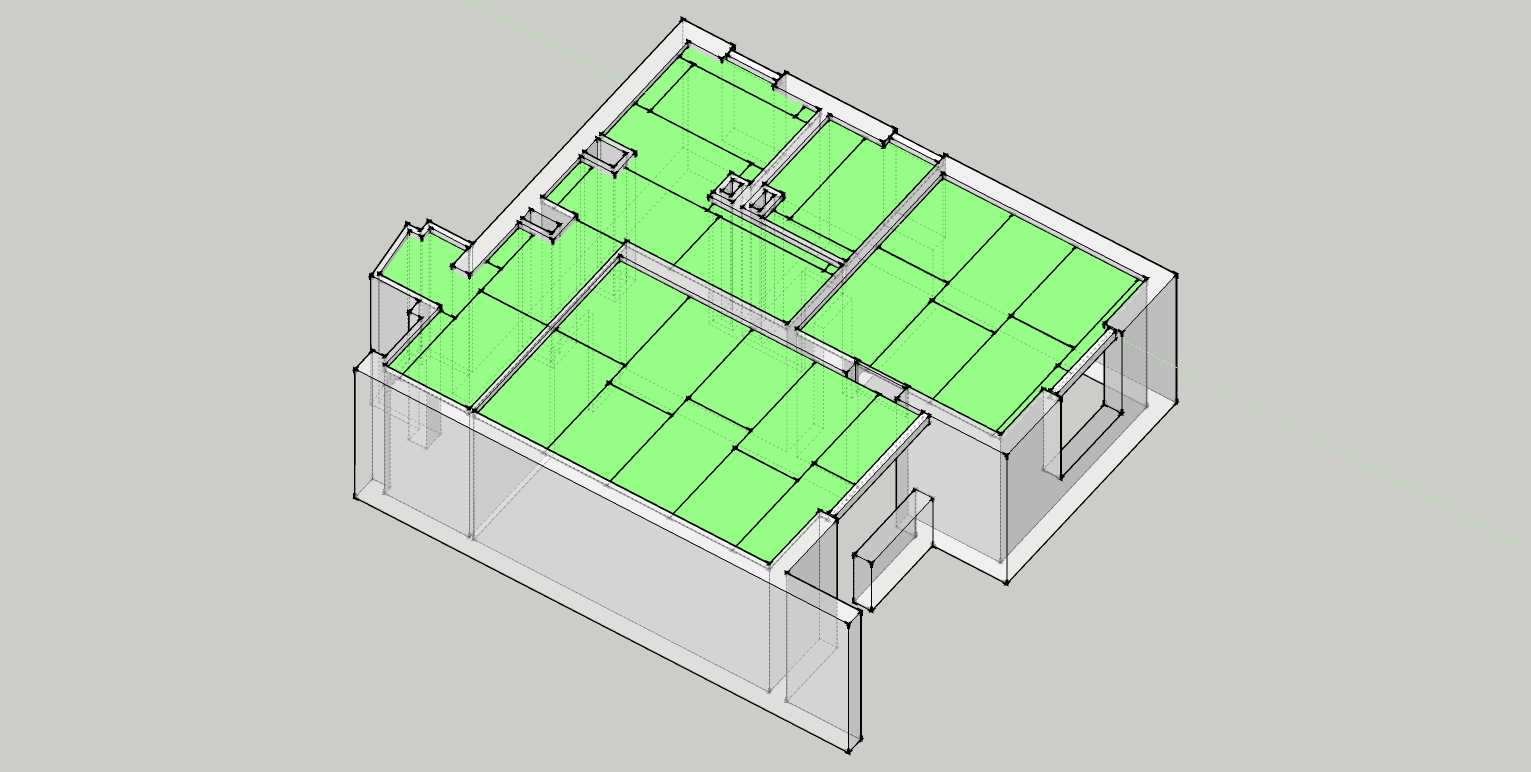
\includegraphics[width=\textwidth]{gipszkarton.png}
\caption{Gipszkarton lapok elosztása}
\label{fig:gipszkarton}
\end{figure}
\begin{figure}[h]
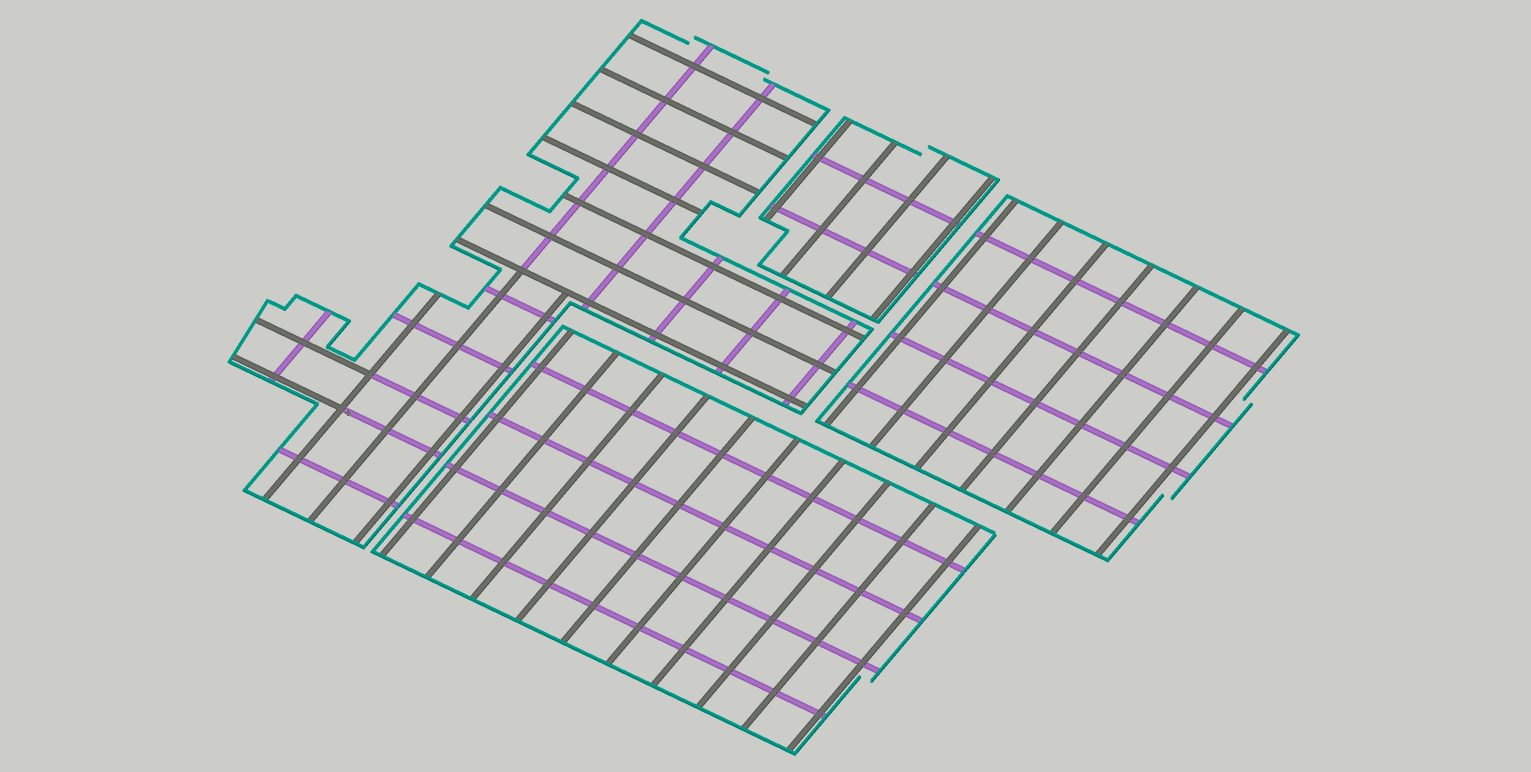
\includegraphics[width=\textwidth]{gipszkarton_vazszerkezet.png}
\caption{Gipszkarton vázszerkezet}
\label{fig:gipszkarton_vaz}
\end{figure}
\begin{figure}[h]
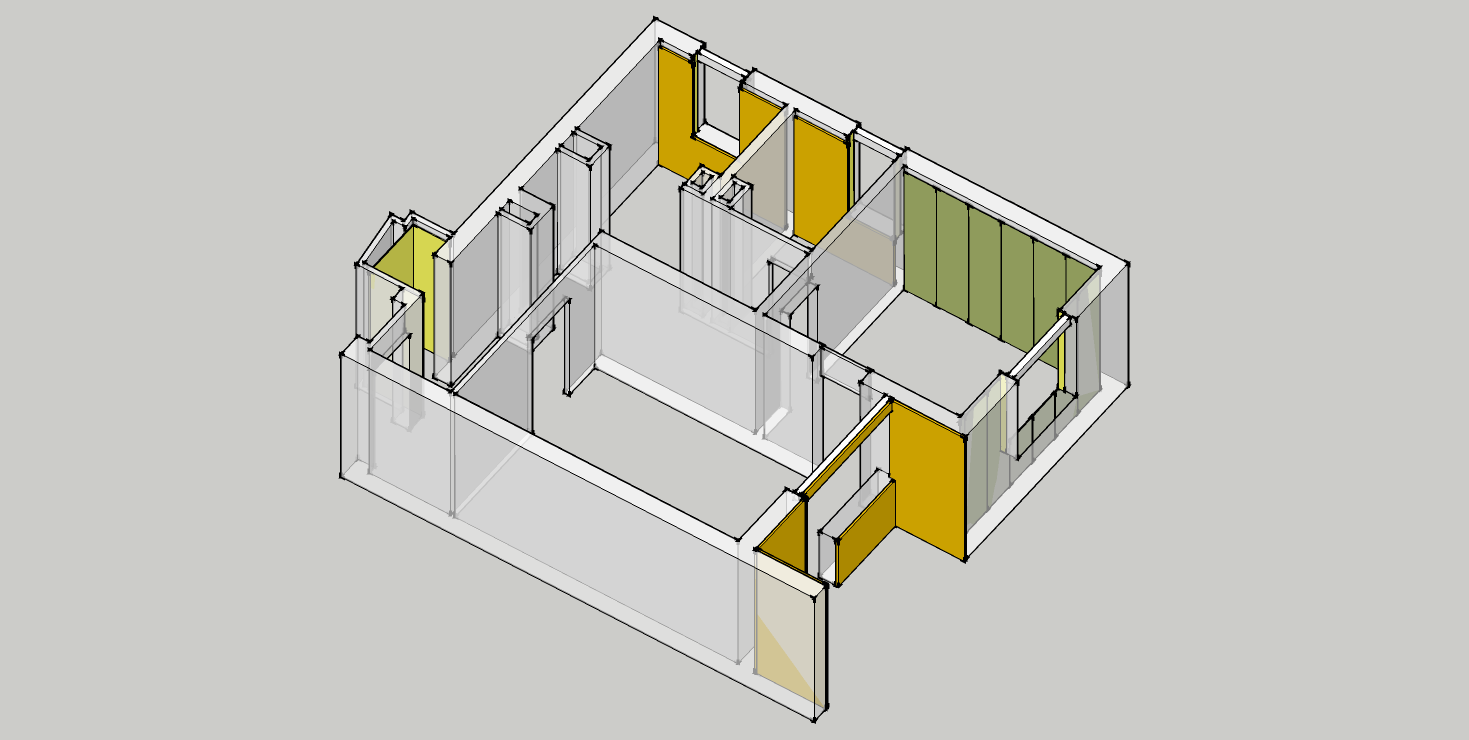
\includegraphics[width=\textwidth]{szigeteles.png}
\caption{Utcai falak és közműakna falak szigetelése}
\label{fig:szigeteles}
\end{figure}

\clearpage
\phantomsection\addcontentsline{toc}{section}{\listfigurename}
\label{sec:abrajegyzek}
\listoffigures

\clearpage
\phantomsection\addcontentsline{toc}{section}{\listtablename}
\label{sec:tablajegyzek}
\listoftables

\clearpage
\phantomsection\addcontentsline{toc}{section}{\indexname}
\label{sec:targymutato}
\printindex

\clearpage
\phantomsection\addcontentsline{toc}{section}{\appendixname}
\label{sec:melleklet}
%\input{./melleklet.tex}

\end{document}
